\documentclass[12pt, titlepage]{article}
\usepackage[utf8]{inputenc}
\usepackage{amssymb}
\usepackage{amsmath}
\usepackage{amsfonts}
\usepackage{indentfirst} % Indent paragraph
\usepackage[norule,bottom]{footmisc} % Footing options
\usepackage[justification=centering,textfont={sc},labelfont={rm}]{caption}

% Page settings
\usepackage[left=1.5in, right=1.5in, top=1in, bottom=1in]{geometry}
\usepackage{setspace}
\onehalfspacing
%\doublespacing  % \singlespacing 

% Font
\usepackage{times} % times, palatino, lmodern, tgtermes
									 % bookman, charter, tgschola, pslatex

% Tools
\usepackage{beamerarticle} % Not sure
\usepackage{todonotes} % Todos
\usepackage{appendix} % Appendix
\usepackage{array,booktabs,longtable,rotating} % Tables
%\usepackage{lineno}+ %\linenumbers

% Sections, captions, etc.
\usepackage{sectsty} % Section styles
\sectionfont{\centering\scshape} % \normalfont
\subsectionfont{\itshape}
\renewcommand{\thesection}{\arabic{section}.}
\renewcommand{\thesubsection}{\thesection\arabic{subsection}.}

% Line numbers

% Links
\usepackage{hyperref}
%\hypersetup{%
%  colorlinks=false,% hyperlinks will be black
%  linkbordercolor=red,% hyperlink borders will be red
%  pdfborderstyle={/S/U/W 1}% border style will be underline of width 1pt
%}

% Position tables {here, top, bottom, page}
\makeatletter
\def\fps@table{htbp}
\makeatother

%% ... at the end of paper

% Create new minipage environment for notes 
% at the bottom of tables or figures
\newenvironment{tablenotes}[1][Note:]{
  \vskip 1.8ex
  \begin{minipage}{\textwidth}\itshape\footnotesize{#1}
} {\end{minipage}}


% Graphics
\usepackage{graphicx,grffile}
\makeatletter
\def\maxwidth{\ifdim\Gin@nat@width>\linewidth\linewidth\else\Gin@nat@width\fi}
\def\maxheight{\ifdim\Gin@nat@height>\textheight\textheight\else\Gin@nat@height\fi}
\makeatother
% Scale images if necessary, so that they will not overflow the page
% margins by default, and it is still possible to overwrite the defaults
% using explicit options in \includegraphics[width, height, ...]{}
\setkeys{Gin}{width=\maxwidth,height=\maxheight,keepaspectratio}
% set default figure placement to htbp
\makeatletter
\def\fps@figure{htbp}
\makeatother

\usepackage{natbib}% plainnat
\bibliographystyle{abbrvnat}
\setcitestyle{authoryear,open={(},close={)}}
%\bibliographystyle{aer}


\setlength{\emergencystretch}{3em}  % prevent overfull lines
\providecommand{\tightlist}{%
  \setlength{\itemsep}{0pt}\setlength{\parskip}{0pt}}



\title{Incentives for Public Goods Inside Organizations: Field Experimental
Evidence\thanks{Blasco: Harvard Institute for Quantitative Social Science, Harvard
University, 1737 Cambridge Street, Cambridge, MA 02138 (email:
\href{mailto:ablasco@fas.harvard.edu}{\nolinkurl{ablasco@fas.harvard.edu}}).
Jung: Harvard Business School, Soldiers Field, Boston, MA 02163 (email:
\href{mailto:oliviajung@gmail.com}{\nolinkurl{oliviajung@gmail.com}}),
Lakhani: Harvard Business School, Soldiers Field, Boston, MA 02163, and
National Bureau of Economic Research (email:
\href{mailto:k@hbs.edu}{\nolinkurl{k@hbs.edu}}). Menietti: Harvard
Institute for Quantitative Social Science, Harvard University, 1737
Cambridge Street, Cambridge, MA 02138 (email:
\href{mailto:mmenietti@fas.harvard.edu}{\nolinkurl{mmenietti@fas.harvard.edu}}).
We gratefully acknowledge the financial support of the MacArthur
Foundation (Opening Governance Network), NASA Tournament Lab, and the
Harvard Business School Division of Faculty Research and Development.
This project would not have been possible without the support of Eric
Isselbacher, Julia Jackson, Maulik Majmudar and Perry Band from the
Massachusetts General Hospital's Healthcare Transformation Lab.}}
\author{Andrea Blasco \and Olivia S. Jung \and Karim R. Lakhani \and Michael Menietti}
\date{Last updated: 22 January, 2018}

\begin{document}
\maketitle
\begin{abstract}
We report results of a natural field experiment conducted at a medical
organization that sought contribution of public goods (i.e., projects
for organizational improvement) from its 1200 employees. Offering a
prize for winning submissions boosted participation without affecting
the quality of the submissions. The effect was consistent across gender
and job type. We posit that the allure of a prize, in combination with
mission-oriented preferences, drove participation. Using a simple model,
we estimate that these preferences explain about a third of the
magnitude of the effect. We also find that the opportunity of winning
financial resources to lead one's own project implementation had a
negative effect on participation. These results were sensitive to the
solicited person's gender.

\smallskip\noindent 
JEL Classification: D23; H41; M52.

\smallskip\noindent 
Keywords: innovation contest; free rider problem; social preferences; altruism; idea generation; organization of work.
\end{abstract}


\clearpage

\section{Introduction}\label{introduction}

Productivity in modern organizations depends on the use of common
resources. These imply that targeted interventions -- improvements,
solutions to common problems -- may have public good effects for the
whole organization. For example, actions taken to improve the workplace
environment or information flow within the organization may increase
productivity and job satisfaction of everyone. Identifying these
opportunities, however, can be difficult. Managers may lack the
information to obtain the desired results. And organizations may be
better off encouraging workers to divide their time between these
``organizational tasks'' and regular production tasks (i.e., tasks with
no public good effects).

From an economics perspective, motivating workers to do organizational
tasks may be challenging. First, it may be difficult to monitor progress
in organizational work and, therefore, offer the worker conventional
contractual incentives tied to performance (like those in the
principal-agent literature). Second, given the public good effects,
workers may view organizational work made by others as a substitute for
their own work and may be tempted to ``free ride'' on their peers.
Finally, even if workers are motivated to act, their interventions may
demand more resources than just one's effort or time.

This article investigates how an organization-wide \emph{internal
contest} -- a competition among workers of the same organization -- may
successfully overcome these problems and foster the provision of public
goods inside organizations. Internal contests are increasingly popular
schemes among firms. There exist many examples of internal contests that
sought to motivate workers of all ranks to identify improvement
opportunities awarding implementation resources to the winning
proposals.\footnote{Apple, for example, uses internal contests among
  store employees to improve the way it sells iPhones in its stores
  (source: ``Apple seeks `pie in the sky' ideas for innovation,''
  \href{http://www.computerworld.com/article/2474058/smartphones/apple-seeks--pie-in-the-sky--ideas-for-innovation}{Computerworld});
  Xerox uses internal contests to change its environmental practices
  (source: ``Xerox employees green ideas save company \$10.2 million,''
  \href{http://www.theguardian.com/sustainable-business/xerox-employees-green-ideas-save}{The
  Guardian}); and AT\&T holds regular contests to collect and develop
  new product ideas from its employees (source: ``AT\&T develops
  employee ideas for innovation,''
  \href{http://blogs.wsj.com/cio/2014/11/12/att-develops-employee-ideas-for-innovation}{The
  Wall Street Journal}).} Economists seem to agree that internal
contests (or tournaments) may have an incentive effect on workers
allocating resources efficiently.\footnote{See: \citet{lazear1981rank};
  \citet{green1983comparison}; \citet{nalebuff1983prizes}; and
  \citet{mary1984economic}.} However, much of the theoretical and
empirical literature on the topic presumes the absence of public good
effects among competitors; in the presence of which contests may no
longer be effective solutions \citep{drago1988incentive}.

Drawing from the literature on public goods, we hypothesize three main
ways in which internal contests that seek workers' contributions to
public goods can remedy the incentives: (1) the competition for an
individual prize to the best proposal generates two opposing
externalities: the positive externality of the public good effect and
the negative externality on the probability of winning a prize of the
others. The concomitant presence of these opposing externalities
mitigates the free riding incentive \citep{morgan2000financing}; (2) the
competition awards implementation resources to the best projects, thus
giving workers the opportunity of influencing the allocation of
collective resources towards preferred interventions (e.g., obtaining
implementation money for own projects); and (3) the contest, beyond
being a competition, draws the attention of employees to relevant
organizational needs triggering voluntary contributions out of
underlying motivations towards helping the organization achieve its
goals \citep{besley2005competition, rotemberg2006altruism}.\footnote{According
  to \citet{besley2005competition}, ``Workers are typically motivated
  agents, i.e., agents who pursue goals because they perceive intrinsic
  benefits of doing so. There are many examples -- doctors who are
  committed to saving lives, researchers to advancing knowledge, judges
  to promoting justice, and soldiers to defending their country in
  battle.''}

In this study, we investigate empirically the relative effectiveness of
these incentives to better understand how organization-wide contests can
foster contributions to public goods inside organizations. We use a
\emph{natural field experiment} to compare the responses of staff
members of a medical organization who are exposed to four different
``solicitation'' treatments -- contest announcements -- seeking projects
for organizational improvement. These are: (1) a solicitation treatment
(PRIZE) announcing the opportunity of winning a prize for the best
proposals; (2) a solicitation treatment (WPLACE) announcing a generic
opportunity of improving the workplace; (3) a solicitation treatment
(PCARE) announcing a generic opportunity of improving the care of
patients; and (4) a solicitation treatment (FUND) announcing the
opportunity of obtaining implementation money to lead one's own
improvement project.

The empirical context for the experiment is the Massachusetts General
Hospital's (MGH) Corrigan Minehan Heart Center (simply referred to as
the ``Heart Center'') a prominent medical organization in the United
States and a teaching hospital of the Harvard Medical School. The health
care delivery context is particularly relevant as the need for
organizational improvement and innovation is vastly noted
\citep{cutler2012reducing}. In addition, health care professionals are
commonly seen as willing to step beyond the boundaries of their
contractual duties to offer better care \citep{delfgaauw2005dedicated},
which makes the comparison of different incentives towards a public good
especially relevant and interesting.

The subject pool was the entire population of the Heart Center
consisting of over 1,200 staff members including physicians, nurses, and
administrative staff. The intervention was associated with an internal
contest aimed to improve the operations of the organization, in the
spirit of ``open innovation'' discussed in
\citet{terwiesch2008innovation}, \citet{lakhani2013prize}, and
\citet{glaeser2016predictive}. The contest solicited employees to submit
project proposals describing an existing problem and providing a
solution to address the problem. After the submission phase, the contest
invited all employees to read and rate each proposal on a five-point
scale. The winning proposal would receive funding for implementation,
implying additional costs and responsibilities from making a winning
proposal (e.g., providing further guidance or a direct involvement in
implementation).

Our solicitation treatments were randomly assigned to each staff member,
thus allowing us to obtain causal estimates of the effect of different
solicitation strategies on two main outcomes: (a) the decision to submit
a proposal and engage in an organizational improvement task and (b) the
quality of the submissions as measured by over 12,000 peer ratings and
by the contest organizers (``the management'').

We further check the effects on employee participation of differences in
preferences or other characteristics associated with the employee's
profession, gender, and position inside the organization. The presence
of sorting effects based on the gender, for example, may impact on the
extent and type of public goods provided, complicating the analysis of
the incentives substantially.

As we shall discuss in Section \ref{results}, our solicitation
treatments produce significant effects on employee participation in the
contest, with small and insignificant effects on the quality of the
proposals. In particular, our findings suggest that: (1) the opportunity
of winning a prize dominates all other incentives; (2) the opportunity
of leading implementation of one's own submitted project proposal, a
non-production task, is the least effective incentive and seems to be
perceived more as a cost than a reward; (3) the increase in
participation rates associated with the announcement of a prize is
without lowering the quality of submissions; and using a simple linear
public-good model, we estimate that (4) responses to the prize incentive
may go beyond the extrinsic value of the prize, consistently with our
theory of prizes as means to internalize public goods.

In addition, by looking at the sorting by gender, profession, and
position inside the organization, we find that: (5) solicitation
treatments with mission-oriented incentives may result in responses that
appear sensitive to the gender of the solicited person (women's response
to solicitations for improving patient care is higher than men's); and
(6) gender differences in preferences, such as competitive inclinations
or risk aversion, may not exert great influence on responses of workers
to the competition-for-prizes incentive (women's and men's response to
solicitations for prizes are the same).

The implications of these results for the provision of public goods
inside organizations are discussed in Section
\ref{summary-and-conclusions}.

\section{Literature}\label{literature}

Economists have long recognized that contests may have an incentive
effect for work inside organizations
\citep{lazear1981rank, green1983comparison, nalebuff1983prizes, mary1984economic}
for which there exist consistent findings across many different
empirical settings, including sport competitions
\citep{ehrenberg1990tournaments}, production competitions in firms
\citep{knoeber1994testing, terwiesch2008innovation}, and more recently
online competitions
\citep{boudreau2011incentives, boudreau2016performance}. We expand on
the existing literature by providing, and examining empirically, a novel
rationale for contests inside organizations: give incentives to workers
to do organizational tasks (tasks with public good effects for the
organization). Much of the existing contest literature in labor
economics presumes indeed that agents are motivated to compete solely on
the basis of the utility derived by owning one of the prizes. Less
attention has been devoted to situations in which a competitor's
performance generates public good effects for the other competitors, and
the whole organization.

To be sure, free riding incentives inside organizations have been widely
studied in labor economics, especially in the context of team production
\citep{erev1993constructive, hamilton2003team, boning2007opportunity, gibbs2014field}.
However, our study differs from much of the existing literature in that
it focuses on an individual competition where the team component is
missing. That is, the public good dilemma comes from externalities
towards anyone in the organization, not just a set of identified team
members. It follows that one can remove from consideration conventional
team dynamics such as peer pressure, monitoring, reciprocity among team
members, and other kinds of social interactions that have been shown to
affect behavior in the presence of free riding incentives.

Our study is also related the literature in public economics that
studies prize-based mechanisms to foster the provision of public goods.
\citet{morgan2000funding} appears to be the first to note that
fixed-prize lotteries -- a special case also known as ``Tullock''
contest -- are widely used tools among non-profit fundraising firms,
showing conditions under which these may increase the provision relative
to voluntary contributions. This insight has spurred much attention in
public economics with several studies testing this idea empirically
\citep[see][ for a survey]{vesterlund2012voluntary}. However, as noted
by Vesterlund, the existing evidence on the profitability of lotteries
for charities is only mixed. Our work extends the existing literature on
the topic by focusing on an organizational setting where monetary
contributions are replaced by effort and the ``greater good'' is helping
the organization achieve its goals. Within this context, we find
evidence that fixed-prize contests are a profitable tool to foster
public good effects inside firms.

Finally, our work provides support to the incentive effect of
mission-oriented preferences -- inner satisfaction from helping the
organization achieve its goals --
\citep{akerlof2005identity, besley2005competition, delfgaauw2005dedicated, delfgaauw2008incentives, prendergast2007motivation, rotemberg2006altruism}
and social preferences at work
\citep{bandiera2005social, bandiera2008social, bandiera2013team, dellavigna2016estimating}.
According to this perspective, workers are motivated agents. They do
their work because they care about their co-workers, employers, and
customers. Theoretical models suggest different ways in which managers
can exploit these intrinsic motivations to raise individual levels of
participation and productivity. Here, we use announcing an internal
contest for organizational improvements to make these motivations
salient. We find that emphasizing mission-oriented motivations has
countervailing effects: positive for women and negative for men. While
this finding is consistent with altruism being an important driver of
effort inside organization, it also suggests that people are sensitive
to the framing and in ways that may be difficult to predict ex-ante.

\section{Analytical framework and
predictions}\label{analytical-framework-and-predictions}

In this section, we conceptualize an internal solicitation for
innovation project proposals to improve the operations of the
organization as a voluntary contribution mechanism for a public good.
Successful proposals are viewed as non-excludable because innovation
leads to improvements for everyone in the workplace (including customers
by increasing the quality and efficiency of the services provided).
Submitting a proposal requires costly effort by employees, such as the
time to identify a problem, form a proposal, write up a concise
description, and the potential for further involvement during proposal
implementation.

Consider a linear model of the utility of a typical employee who
contributes \(x\) and benefits from total contributions of
\(Y=\sum x\):\footnote{functionalform}

\begin{equation} \label{eq:utility}
  u(R,~ Y) =  \gamma Y + \delta x + \frac{x}{Y} R - c x.
\end{equation}

The benefits of contributing derive from three sources. First, there is
an altruistic benefit from the improved workplace, \(\gamma Y\). The
altruistic benefits are the crux of public goods. Only the existence of
an improved workplace is desired and the source of contributions is
irrelevant. Thus, everyone would prefer to free ride on others' efforts.
Second, participants have some chance of winning the contest and can
expect to derive benefits from the prizes, \(\frac{x}{Y} R\), where, for
simplicity, all efforts have an equal chance of being selected as the
winner, as in \citet{morgan2000financing}. The personal reward \(R\) can
be thought of as a pecuniary prize, but it could also be an increase in
prestige or recognition or any combination of the above. Finally,
employees may have an egoistic motivation for contributing ``per se,''
regardless of winning and the effect on others, which is captured by
\(\delta x\). This includes the case in which workers may derive a
personal satisfaction from contributing personally to the organization,
often called warm glow preferences for giving \citep{andreoni1995warm}.
Since we cannot observe the distinction between altruistic and warm-glow
motives in our empirical setup, we are going to impose later that these
preferences are such that \(\delta=0\).

Contributors incur some cost from developing and submitting a proposal,
\(c x\). If there are \(n\) employees the public goods dilemma arises
when \(\gamma+\delta < c < n\gamma+\delta\). Then no individual would
contribute without a reward as costs exceed individual benefits, but
everyone would be better off if everyone contributes.

Suppose contributing a proposal is a discrete choice by employees. An
employee can either contribute a single proposal \(x=1\) and receive
utility of

\begin{equation}
    u_1 = \gamma \hat Y + \delta + \sum_{k=1}^{n}\Pr(Y=k)\frac{R}{k}  - c, 
\end{equation}

where \(\hat Y\) denotes the expected level of contributions and
\(\Pr(Y=k)\) is the probability of having \(k\) total contributions. Or
they can contribute nothing \(x=0\) and receive utility of

\begin{equation}
  u_0 = \gamma (\hat Y - 1).
\end{equation}

If there are \(n\) employees, then the unique symmetric mixed-strategy
equilibrium is for each employee to contribute a proposal with
probability \(p>0\). After using the binomial probability for
\(\Pr(Y=k)\), the payoff-equating condition to find a mixed-strategy
equilibrium is:

\begin{equation} \label{eq: mixed-strategy}
  \frac{1- (1-p)^{n}}{n p} = (c- \gamma - \delta) / R.
\end{equation}

This equation admits one single solution \(p^*\) which cannot be
expressed explicitly. Using a first order Taylor expansion around \(p\),
the equilibrium probability can be approximated as follows:

\begin{equation} \label{eq: probability}
  p^*  \approx \frac{2 (R- c+\gamma +\delta )}{(n-1) R}. 
\end{equation}

The analysis of the above model is used to derive the following
predictions.

\begin{enumerate}
\def\labelenumi{\arabic{enumi})}
\item
  The probability of contributing a proposal to improving the
  organization is zero when the prize for winning is sufficiently small
  relative to the individual cost of effort minus the preference for the
  public good (i.e., \(R< c-\gamma +\delta\)).
\item
  The probability of contributing a proposal to improve the organization
  increases with the value of the prize for winning.
\item
  The probability of contributing a proposal to improve the organization
  increases with the extent of individual preference for the public good
  (\(\gamma+\delta\)).
\end{enumerate}

Now suppose that the public good \(Y\) constitutes the sum of innovation
projects to improve the organization. Imagine that the quality of each
project is randomly drawn from a discrete distribution, the same for
every contributor (every employee who contributes is assumed to be
equally likely to come up with a useful idea). Each proposal can be of
high quality with probability \(\nu\) and of low quality with
probability \(1-\nu\). If a proposal is of low quality, then the value
for the organization is normalized to zero. The quality of proposals is
learned only after the agent paid the cost of effort. Now the
equilibrium public good \(Y\) is not deterministic but follows a
binomial distribution with average \(E[Y] = p^{**} \nu n\), where the
equilibrium probability \(p^{**}\) can be derived as before with the
only difference being that it is also an increasing function of the
probability \(\nu\). This leads to the following prediction.

\begin{enumerate}
\def\labelenumi{\arabic{enumi})}
\setcounter{enumi}{3}
\tightlist
\item
  If the public good depends on the quality of each contribution and
  every agent is equally likely to make a proposal of high quality, then
  the higher the probability of contributing, the higher is the average
  public good.
\end{enumerate}

This framework can be extended to the case of individuals with
heterogeneous costs. In the appendix, we explicitly consider the case of
two types of individuals with different marginal costs of effort that
form two groups of equal size. The symmetric mixed-strategy equilibrium
is then characterized by the vector of probabilities of contributing
with a proposal \((p_1^\star, p_2^\star)\). Here, the analysis of the
payoff-equating conditions for the mixed-strategy equilibrium shows that
the higher the marginal cost of effort minus preference for
contributing, the lower the equilibrium probability of individuals
(i.e., \(p_1^\star > p_2^\star\) when \(c_1 < c_2\), and vice versa).
This leads the final prediction.

\begin{enumerate}
\def\labelenumi{\arabic{enumi})}
\setcounter{enumi}{4}
\tightlist
\item
  If individuals have heterogeneous costs, then the probability of
  contributing a proposal to improve the organization is higher for
  agents with lower costs (positive sorting).
\end{enumerate}

\section{Experimental Design}\label{experimental-design}

\subsection{The context}\label{the-context}

The Heart Center is a leading academic medical center specializing in
clinical cardiac care and research in the United States. Founded more
than a hundred years ago, the Heart Center serves thousands of patients
every year, occupies more than 35,000 square feet of office space, and
employs more than 1,200 people (nurses, physicians, researchers,
technicians, and administrative staff) scattered across several
buildings on the Massachusetts General Hospital's main campus in
downtown Boston and a few other satellite locations.

The study was in cooperation with the Heart Center's launch of the
Healthcare Transformation Lab (HTL),\footnote{\url{http://www.healthcaretransformation.org}}
an initiative aimed at developing innovative health care process
improvements to enhance the health care safety and delivery of the
hospital. The launch of the HTL was accompanied by the announcement of
an internal ``innovation contest,'' called the Ether Dome
Challenge\footnote{The name is taken from a historical place on MGH's
  main campus where the first public surgery using anesthesia was
  demonstrated in 1846.} that sought to engage all staff members to
participate.

The communication around the innovation contest highlighted the
opportunity for staff to help in the selection process of the ideas and
a commitment by the Heart Center Management that the leading ideas would
be provided appropriate resources so that they could be implemented. The
announcement on the contest's website read:

\begin{quote}
``If you've noticed something about patient experience, employee
satisfaction, workplace efficiency, or anything that could be improved;
if you've had an inspiration about a new way to safeguard health; or if
you simply have a cost-saving idea, then now is the time to share your
idea.''
\end{quote}

\begin{figure}
\centering
\caption{Timeline of the innovation contest}
\label{timeline}
\includegraphics{figures/methods_timeline-1.pdf}
\end{figure}

The innovation contest was divided into three main phases (Figure
\ref{timeline}): submission, the peer evaluation, and implementation
phase.

The first was a four-week submission phase. All staff members were
encouraged to identify one or more organizational problems and submit
proposals addressing them. Employee participation was voluntary. All
project submissions were done online via the website of the contest.
There was no limit to the project proposals to submit (proposals could
cover any issue within the organization, as described above), but each
proposal was limited to approximately 300 words to lower the costs of
entry and encourage broader participation. To ensure that treatment
effects could be isolated, identified, and matched to participants, team
submissions were not permitted. Limiting submissions to individual
participation allowed us to match each submitter's characteristics to
the randomly assigned treatment. It also lowered incentives to
communicate or exchange information with other employees. Also, the
website was designed to not provide any information about the status of
the contest during the submission period. In this way, decisions could
not be easily influenced by the perceived popularity of the contest or
previous submissions.

It followed a two-week peer evaluation phase in which all staff members
were invited to rate the merit and potential of submitted proposals on a
five-point rating scale. All evaluations were done online on the website
of the contest. Each signed-up employee was shown a list of anonymized
proposals to read and rate. Proposals were presented at random in
batches of 10 each. Each proposal was described by a title, a main
description of the problem to solve, and the proposal. Voting was then
introduced by the following text: ``Rate this idea'' followed by the
rating scale: 1-low; 2; 3; 4; 5-high. Ratings were kept confidential and
the website did not provide any feedback or any other kind of additional
information that might have influenced individual judgment until the
voting phase was over. Evaluators were free to decide how many (and
which) proposals to rate. Since these were presented in a random order,
every proposal had on average the same exposure to people asked to rate
its quality. Evaluators were offered a limited edition T-shirt as a
compensation for the effort in voting.

In the final implementation phase, employees having submitted proposals
highly rated by peers and judged as particularly promising by the HTL
staff were invited to submit a full proposal detailing plans for
implementation. Following evaluation by MGH senior leadership, top
proposals were selected to receive support and funding for
implementation. This final phase took a few months to complete,
essentially the time necessary to select and implement the best
projects.

\subsection{The design}\label{the-design}

Within this context, we designed a \emph{natural field experiment}
(staff members are unaware of being part of an experiment). The basic
idea of the experiment was to randomize the content of the communication
announcing the innovation contest to all staff members. The start of the
submission phase was indeed announced to everyone in a series of
personalized emails. A direct message was sent to each contact in the
list of employees' emails from our subject pool.

The content of this communication with a placeholder for our
solicitation treatment is reported below (a copy of the exact email is
in the Appendix).

\begin{quote}
Dear Heart Center team member,

\textbf{Submit your ideas to {[}TREATMENT HERE{]}}

The Ether Dome Challenge is your chance to submit ideas on how to
improve the MGH Corrigan Minehan Heart Center, patient care and
satisfaction, workplace efficiency and cost. All Heart Center Staff are
eligible to submit ideas online. We encourage you to submit as many
ideas as you have: no ideas are too big or too small!

Submissions will be reviewed and judged in two rounds, first by the
Heart Center staff via crowd-voting, and then by an expert panel.
Winning ideas will be eligible for project implementation funding in the
Fall of 2014!
\end{quote}

The first paragraph of the above message was randomized into \emph{four}
different solicitation treatments (the exact words are in Table
\ref{experimental-design}), thus creating as many treatment groups of
equal size (Table \ref{experimental-design}). The first group was given
a solicitation treatment (PRIZE) announcing the innovation contest as an
opportunity to win individual prizes (iPad mini's) for top submissions.
The second group was given a solicitation treatment (FUND) announcing
the contest as an opportunity to win a \$20,000 budget for developing
their project proposals. The other groups received solicitation
treatments announcing the contest as an opportunity to improve the
health care of their patients (PCARE) or the workplace (WPLACE).

\begin{table}
\centering
\caption{Experimental design}
\label{experimental-design}
\begin{tabular}{@{}lp{5cm}>{\raggedright}rr}
  \\[-1.8ex]\hline \hline \\[-1.8ex]
 & \multicolumn{1}{c}{\emph{Solicitation treatment:}}
                        & \multicolumn{2}{c}{\emph{Employees:}}\\
                        \cmidrule(lr){2-2}\cmidrule(lr){3-4} &   & freq. & \% \\ 
  \hline \\[-1.86ex]
PRIZE & Submit your ideas to win an Apple iPad mini & 312 & 25 \\ 
  [1.8ex] FUND & Submit your ideas to win project funding up to \$20,000 
            to turn your ideas into actions & 308 & 25 \\ 
  [1.8ex] PCARE & Submit your ideas to improve patient care at the Heart Center & 310 & 25 \\ 
  [1.8ex] WPLACE & Submit your ideas to improve the workplace at the Heart Center & 307 & 25 \\ 
  [1.8ex] Total &  & 1237 & 100 \\ 
   \\[-1.8ex]\hline \hline \\[-1.8ex]
\end{tabular}
\end{table}

A sample size of more than 300 units for each treatment group ensured a
sufficiently high statistical power based upon standard power
calculations on the difference of proportions. In testing the difference
of proportions between any two treatments, the probability of type-I
errors was slightly below \(0.80\) for \emph{small} differences at 5
percent significance level but higher than \(0.80\) for \emph{medium}
and \emph{large} differences at the more stringent 1 percent
significance level.\footnote{The definition of small, medium and large
  differences is given by \citet{cohen1992power}; e.g., a difference of
  5 percentage points of the pair \((0.05, 0.10)\) is considered a small
  effect: see \citet{cohen1992power} p.~158.}

Also, note the lack of a traditional ``control'' treatment in this
study. Since the experiment was run in a workplace, we were constrained
to carry out treatments having equal chances of being successful. This
prevented us from having a `null' treatment with no personalized
incentives messaging as a control group. Indeed, the analysis focused on
multiple comparisons of several unordered discrete treatments (e.g.,
prizes vs funding vs framing).\footnote{Nevertheless, if we were to
  think of one treatment as the benchmark against which to compare the
  others, the FUND treatment would be our best candidate because giving
  information about the size of available funding is the default option
  for announcing grant programs and was part of the HTL's initial design
  before our cooperation in the experiment.}

These solicitation messages were sent three times: at the launch of the
submission phase, eight days from the launch and two days before the end
of the submission phase of the challenge.

The website of the innovation contest had supporting information about
the available prizes, funding, and timing of the initiative. The website
also required an institutional email address to login. Using this
feature, we designed the website graphics and layout to reinforce the
effect of the announcement: the headings, background images, a short
video, and the space just below a ``submit your ideas'' button were
designed to show the exact same first paragraph of the solicitation that
the employee received by email (i.e., text in Table
\ref{experimental-design}).

The MGH management and the HTL staff members were blind to group
assignment, which prevented potential bias in the communication of the
innovation contest that was not under our direct control. We also made
an effort to create a ``safe'' environment for employees submitting
proposals by making clear (in the application form) that the identity of
the proponents was going to be kept private unless the employee
self-identified, so that management could not identify workers without
their consent.

Finally, we relied only on official channels for communication to
strengthen the effect of the announcement and signal legitimacy of the
contest. Each employee received the same exact solicitation email three
times: at the launch, eight days from the launch and two days before the
end of the submission phase of the challenge. Starting from the second
week of the submission phase, information booths, flyers, and posters
were used to encourage everyone to take part in the event and respond to
the email solicitation. These flyers and posters were based on a
generic, undifferentiated version of the solicitation email without the
text of the treatments.

\section{Data}\label{data}

Our subject pool is the entire population working at the Heart Center as
of the end of 2014, a total of 1,237 individuals. For each individual,
we have administrative data on the gender, the type of profession, and
whether they had a fixed office location or not. Additional,
complementary data are available for a limited group of 378 employees
(31 percent). These extra data have self-reported information about
employees' demographics, such as age and years of tenure at the Heart
Center, that were obtained from an online survey that was run about two
months before the launch of the innovation contest.

We report summary statistics for the different variables by solicitation
treatment (Table \ref{summary-statistics}), showing that these are
statistically balanced across groups. These also show that the large
majority (72 percent) of employees in our sample are women. This is due
to the high fraction of workers being nurses (52 percent) and the
presence of a gender separation by profession with nurses being
predominantly women (92 percent).

Nursing workers constitute about half of the sample, and the rest is
split almost equally between physicians and administrative workers.
Though we do not have data on income, there exist large differences in
earnings across these professions. According to the United States Bureau
of Labor Statistics, the median annual wage of a physician was \$187,200
in 2015, which is about 60 percent higher than the that of a registered
nurse (\$67,490) and about 70 percent higher than that of a laboratory
technician (\$38,970). It follows that, if staff members are motivated
by the extrinsic value of the prize alone, one should expect large
differences in participation rates across profession.

Finally, it is also important to remark that only half of the employees
(\(53\) percent) have fixed office locations, as they may be on duty in
multiple wards. However, more senior staff tend to have a fixed
location. So, within each profession, this measure can be viewed as a
proxy for the employee's position or status inside the organization.

\begin{table}
\centering
\caption{Summary statistics by treatment}
\label{summary-statistics}
\begin{tabular}{@{}lccccccc}
  \\[-1.8ex]\hline \hline \\[-1.8ex]
 & \multicolumn{4}{c}{\emph{Assigned treatments:}} 
                        & \multicolumn{2}{c}{\emph{All:}}\\
                        \cmidrule(lr){2-5}\cmidrule(lr){6-7} & FUND & PCARE & WPLACE & PRIZE & \% & Obs. & P-value \\ 
  \hline \\[-1.86ex]
Other & 30 & 30 & 26 & 32 & 29 & 362 & 0.844 \\ 
  MD/Fellow & 19 & 18 & 18 & 18 & 18 & 226 &  \\ 
  Nursing & 51 & 52 & 56 & 51 & 52 & 649 &  \\ 
  [1.86ex] Female & 69 & 70 & 75 & 75 & 72 & 890 & 0.159 \\ 
  Male & 31 & 30 & 24 & 26 & 28 & 347 &  \\ 
  [1.86ex] No office & 50 & 46 & 47 & 45 & 47 & 577 & 0.556 \\ 
  Office & 50 & 54 & 52 & 56 & 53 & 660 &  \\ 
  [1.86ex] 18-25 years old* & 6 & 8 & 8 & 6 & 6 & 24 & 1.000 \\ 
  26-35 years old* & 29 & 29 & 31 & 26 & 29 & 107 &  \\ 
  36-45 years old* & 18 & 19 & 24 & 16 & 22 & 81 &  \\ 
  $>$45 years old* & 44 & 46 & 51 & 45 & 42 & 157 &  \\ 
  [1.86ex] $<$ 10 years tenure* & 40 & 31 & 36 & 37 & 36 & 132 & 0.891 \\ 
  10-20 years tenure* & 26 & 29 & 38 & 28 & 30 & 111 &  \\ 
  20-30 years tenure* & 12 & 19 & 15 & 10 & 14 & 50 &  \\ 
  30-40 years tenure* & 10 & 16 & 15 & 12 & 13 & 48 &  \\ 
  $>$40 years tenure* & 10 & 4 & 8 & 8 & 8 & 28 &  \\ 
   \\[-1.8ex]\hline \hline \\[-1.8ex]
\end{tabular}
\begin{tablenotes}
This table reports the percentage of employees in our sample cross tabulated by the assigned treatment across the gender, profession, whether the employee had a fixed office location, age, and years of tenure at the Heart Center. For each categorical variable, the last column reports the p-value from a Pearson's Chi-squared test with the assigned treatment and the variable. The asterisk $^{\ast}$ indicates non-representative self-reported information obtained from an online survey polling  employees that was run about two months before the launch of the innovation contest.
\end{tablenotes}
\end{table}

\section{Results}\label{results}

\subsection{Submitting project
proposals}\label{submitting-project-proposals}

We first examine treatment differences in participation by looking at
the percentage of employees who made a project submission (Figure
\ref{figure_participation}). Based on the results of the four-week
submission period, we find that, when the solicitation highlights the
opportunity of a prize to be won (PRIZE), employee participation is
considerably higher relative to the other solicitation treatments. In
particular, the proportion of submissions in the PRIZE solicitation
treatment is 7.4 percent, which is 7.4/4.5=1.64 and 7.4/5.2=1.42 times
higher relative to those associated with solicitation treatments
replacing the prize opportunity by a general encouragement to
participate (PCARE, 4.5 percent; and WPLACE, 5.2 percent). The
difference is even more dramatic when the prize opportunity is replaced
by information about available project implementation funding (FUND, 2.3
percent), compared to which the proportion of submissions in the PRIZE
solicitation treatment is 7.4/2.3=3.22 times higher.

\begin{figure}
\caption{Employee participation by solicitation treatment}
\label{figure_participation}
\centering
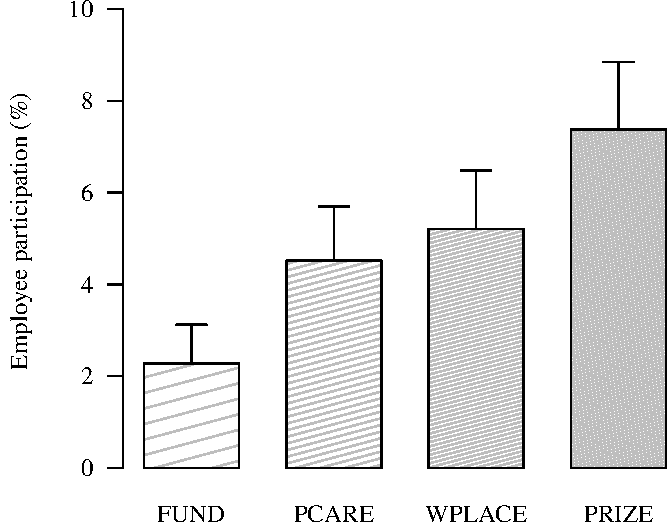
\includegraphics{figures/figure_participation-1.pdf}
\end{figure}

\begin{table}
\centering
\caption{Pairwise difference in participation rates}
\label{pairwise}
\begin{tabular}{@{}lccc}
  \\[-1.8ex]\hline \hline \\[-1.8ex]
 & Lower & Upper & P-value \\ 
  \hline \\[-1.86ex]
PRIZE - FUND & 1.756 & 8.442 & 0.003 \\ 
  PRIZE - PCARE & -0.853 & 6.564 & 0.132 \\ 
  PRIZE - WPLACE & -1.659 & 5.980 & 0.269 \\ 
  FUND - PCARE & -5.092 & 0.605 & 0.124 \\ 
  FUND - WPLACE & -5.931 & 0.053 & 0.055 \\ 
  PCARE - WPLACE & -4.090 & 2.699 & 0.688 \\ 
   \\[-1.8ex]\hline \hline \\[-1.8ex]
\end{tabular}
\begin{tablenotes}
This table reports Wald confidence intervals (95 percent level) for the difference in the proportions of submissions between every two solicitation treatments. The last column reports p-values from a two-sided proportion test where the null tested is that, for a given pair, the proportions of submissions in each group are equal.
\end{tablenotes}
\end{table}

To test to see whether participation rates are statistically different
across solicitation treatments, we use a series of pairwise two-sample
tests of proportions (Table \ref{pairwise}). The analysis reveals that
the positive difference between the PRIZE and PCARE solicitation
treatments is marginally statistically significant (p=0.132); the
positive difference between the PRIZE and WPLACE solicitation treatments
is insignificant (p=0.269); and the positive difference between the
PRIZE and FUND solicitation treatments is statistically significant
(p=0.003). This evidence thus indicates a positive causal effect on
participation of highlighting the prize opportunity compared to a
general encouragement (although only marginally significant) and
announcing available funding.

The analysis of the pairwise comparisons shows further a negative
difference between the FUND and the WPLACE solicitation treatments that
is statistically significant (p=0.055); and a negative difference
between the FUND and the PCARE solicitation treatments that is
marginally statistically significant (p=0.124). This evidence thus
indicates a negative causal effect on employee participation of
highlighting the available funding compared to a general encouragement
to participate. In other words, while a solicitation strategy based on
individual prizes is effective, a solicitation focused on the
opportunity of getting implementation funding alone could harm
participation relative not only to prizes but also to general
encouragements towards improving the workplace.

\begin{figure}
\caption{Submissions over time by solicitation treatment}
\label{figure_dynamics}\centering
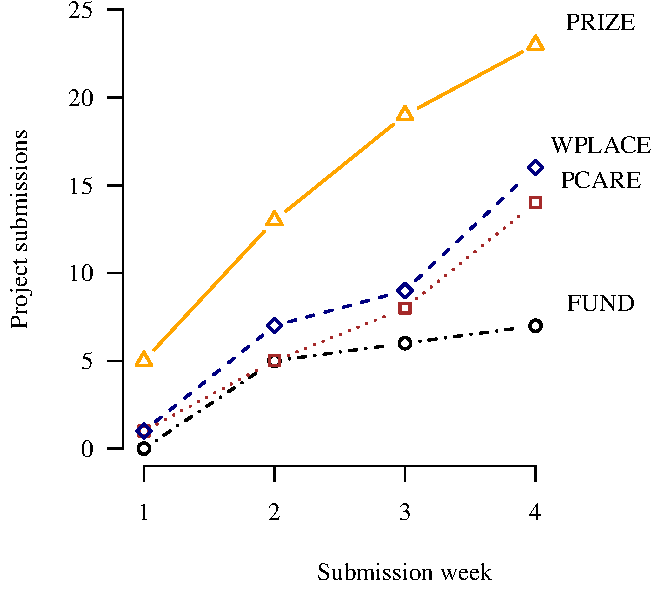
\includegraphics{figures/figure_dynamics-1.pdf}
\end{figure}

We now turn to examining how employee participation evolves over time
(Figure \ref{figure_dynamics}). Though our data may not allow for a
complete analysis of submission dynamics, looking at the overall
submission patterns can be useful for various reasons. In particular, if
employees assigned to different solicitation treatments were sharing
(either face-to-face or electronically) the content of their
solicitation with others, one should expect their participation rates to
converge over time, yielding estimates of the causal effects of a
solicitation treatment biased towards zero. Contrary to these
expectations, Figure \ref{figure_dynamics} shows no evidence of a strong
convergence. Submissions in the PRIZE solicitation treatment are
constantly higher than in the other treatments (except perhaps in the
final week); and, at the same time, submissions in the FUND treatment
are constantly low. These patterns are hence consistent with
communication effects having little, or no, consequences on our
findings, a topic we will discuss in greater detail later (Section
\ref{discussion}).

Another important question related to employee participation is the role
of employee heterogeneity --- i.e., in the benefits from organizational
improvements and the opportunity cost of contributing time and effort.
We, hence, employ a simple regression model to check whether differences
in participation can be explained by differences in the gender,
profession, and organizational role of the employee. The probability of
submitting, \(y_i=1\), is given by

\begin{equation} 
  \label{eq: submit}
    \Pr(y_i=1) = \alpha_0 + \sum_{j} \alpha_{j} \text{SOLICIT}_{ij}
                                    + \text{JOB}_{i} 
                                    + \text{MALE}_{i} 
                                    + \text{OFFICE}_{i}, 
\end{equation}

where \(\alpha_0\) is a constant, \(\alpha_j\) is the causal effect of
the solicitation treatment \(j\) assigned to an employee \(i\)
(\(\text{SOLICIT}_{ij}\)), controlling for the employee's profession
(\(\text{JOB}_i\)), the gender (\(\text{MALE}_i\)), and a dummy for
office location (\(\text{OFFICE}_i\)) that indicates whether the
employee had a permanent office instead of being assigned to a ward.
Note that, in our context, having a fixed office location is highly
correlated with the type of profession.\footnote{Much of the clinical
  staff might be mobile and only half of the employees (\(53\) percent)
  had fixed office locations, as they may be on duty in multiple wards.
  More senior staff tend to have a fixed location. So, within each
  profession, this measure can be viewed as a proxy for status inside
  the organization.} For example, nurses are more likely to being
assigned to a ward than physicians or administrative workers, due to the
nature of their job. Within each profession, however, having a fixed
office location is usually correlated with the hierarchical position
inside the organization. Beyond having a fixed office location per se,
this variable is hence potentially controlling for income and
hierarchical differences occurring within each profession as well.

\begin{table}
\centering
\caption{Probability of submitting proposals}\label{participation ols}
\begin{tabular}{@{\extracolsep{5pt}}lccccc} 
\\[-1.8ex]\hline 
\hline \\[-1.8ex] 
 & \multicolumn{5}{c}{\textit{Dependent variable:}} \\ 
\cline{2-6} 
\\[-1.8ex] & \multicolumn{5}{c}{ $SUBMIT_{ij}=1$ } \\ 
\\[-1.8ex] & (1) & (2) & (3) & (4) & (5)\\ 
\hline \\[-1.8ex] 
 PRIZE & 2.53$^{**}$ & 2.53$^{**}$ & 2.52$^{**}$ & 2.46$^{**}$ & 2.45$^{**}$ \\ 
  & (1.21) & (1.21) & (1.21) & (1.21) & (1.21) \\ 
  & & & & & \\ 
 WPLACE & 0.37 & 0.37 & 0.35 & 0.38 & 0.30 \\ 
  & (1.09) & (1.09) & (1.10) & (1.09) & (1.10) \\ 
  & & & & & \\ 
 FUND & $-$2.57$^{***}$ & $-$2.57$^{***}$ & $-$2.55$^{***}$ & $-$2.49$^{***}$ & $-$2.38$^{***}$ \\ 
  & (0.86) & (0.86) & (0.85) & (0.86) & (0.85) \\ 
  & & & & & \\ 
 Job (nursing) &  & 0.14 &  &  & 1.85 \\ 
  &  & (0.82) &  &  & (1.23) \\ 
  & & & & & \\ 
 Job (MD) &  & $-$0.31 &  &  & $-$1.14 \\ 
  &  & (1.03) &  &  & (1.24) \\ 
  & & & & & \\ 
 Male (yes) &  &  & $-$0.54 &  & $-$0.42 \\ 
  &  &  & (1.33) &  & (1.64) \\ 
  & & & & & \\ 
 Office (yes) &  &  &  & 2.79$^{**}$ & 4.56$^{***}$ \\ 
  &  &  &  & (1.20) & (1.60) \\ 
  & & & & & \\ 
 Constant & 4.84$^{***}$ & 4.78$^{***}$ & 5.00$^{***}$ & 3.35$^{***}$ & 1.97 \\ 
  & (0.61) & (0.66) & (0.73) & (0.75) & (1.25) \\ 
  & & & & & \\ 
\hline \\[-1.8ex] 
Log Likelihood & -5545 & -5545 & -5545 & -5542 & -5540 \\ 
Observations & 1,237 & 1,237 & 1,237 & 1,237 & 1,237 \\ 
\hline 
\hline \\[-1.8ex] 
\end{tabular} 
\begin{minipage}{\textwidth}
\emph{Note:} This table reports OLS estimates with heteroskedasticity robust standard errors in parenthesis. All coefficients are multiplied by 100 to indicate the percentage point change in the probability of submitting. Solicitation treatment dummies are coded to indicate deviations from the overall probability of submitting. The asterisks $^{\ast\ast\ast}$, $^{\ast\ast}$, $^{\ast}$ indicate significance at 1, 5 and 10 percent level, respectively.
\end{minipage}\end{table}

The regression results (Table \ref{participation ols}) show an
insignificant effect on participation associated with an employee's
profession or gender.\footnote{The coefficient for nurses is positive
  and negative for physicians, consistent with sorting. These effects
  are, however, not statistically different from the residual category
  of other workers, as well as from one another.} By contrast, we find a
positive effect associated with the worker having a fixed office
location, as opposed to being assigned to a ward (and the effect size
doubles after controlling for the profession and gender). This evidence
suggests that differences in the employee's hierarchical position inside
the organization, as captured by our office-location regressor, may be a
stronger driver of participation relative to differences in gender and
profession as sometimes assumed by the literature.

The results of the regression model above (Table
\ref{participation ols}) give estimates of the solicitation treatment
differences relative to the overall mean participation and controlling
for baseline characteristics. In theory, these estimates should be more
statistically efficient relative to the pairwise comparisons above
(i.e., by reducing the overall noise associated with baseline
characteristics). We find that, at the 95 level of statistical
significance, employees in the PRIZE solicitation treatment are 2.4
percentage points \emph{more} likely to submit compared to the overall
mean, whereas employees in the FUND solicitation treatment are 2.4
percentage points \emph{less} likely to do so.\footnote{Subtracting
  these two effects gives 4.8 which is the difference in the probability
  of submitting between PRIZE and FUND treatments.} Overall, these
effects are sizable not only in absolute levels but also relative to the
effects of the heterogeneity captured by the other variables.

We now turn to examining treatment interactions involving the employee's
gender and profession (Figure \ref{interactions}).\footnote{We find no
  significant differences for interactions with office location, which
  we do not report for space limitation.} We hypothesize gender
interactions to occur as a result of three main factors: differences in
risk taking, social preferences (willingness to contribute to public
goods), and competitive inclinations. If women prefer to work on
activities that are less risky, more pro-social (e.g., aiming at
improving people's health) and where competition is less intense, then
we should observe significant treatment interactions. Similarly, we
expect treatment interactions associated with the employee's profession
to occur because, for example, the prize opportunity (i.e., the PRIZE
treatment) could be relatively less effective for employees with a
higher income, such as doctors, than the others.

\begin{figure} 
\caption{Employee participation by gender or profession and solicitation treatment}
  \label{interactions}
  \centering
  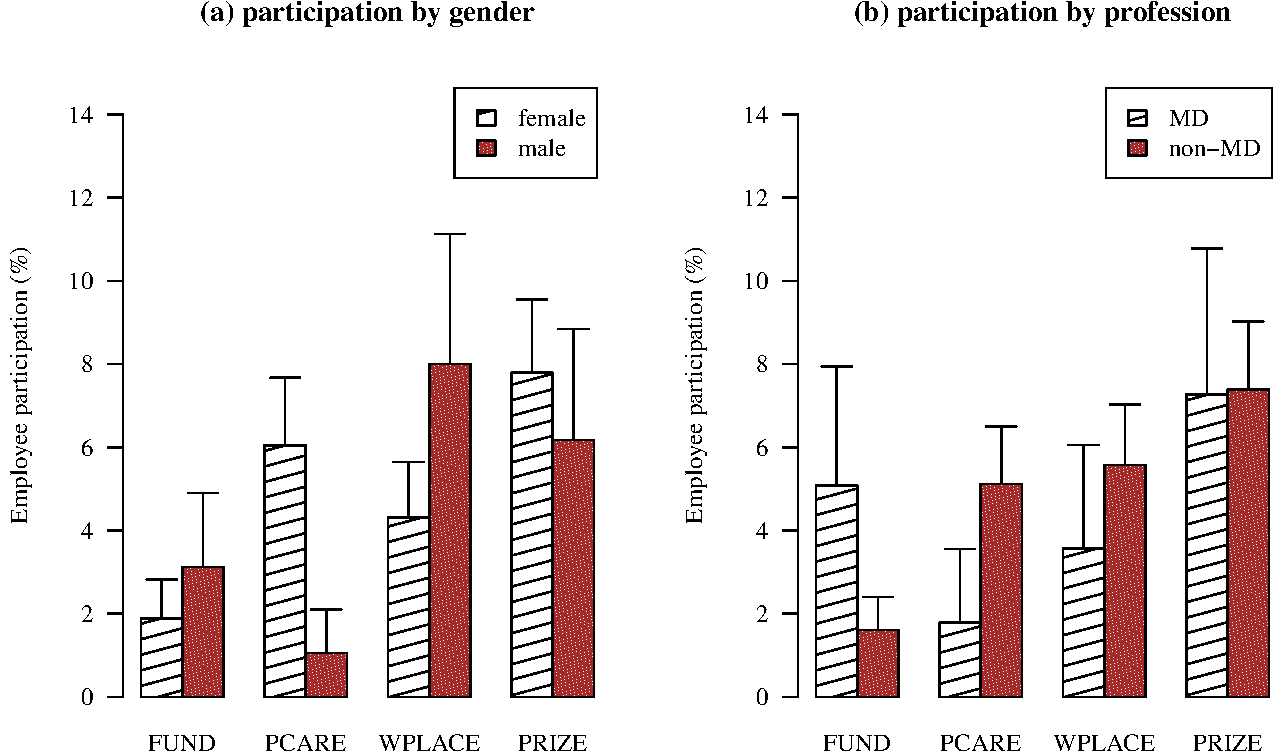
\includegraphics{figures/figure_interactions-1.pdf}
\end{figure}

Examining the proportion of submissions conditional on the gender
(Figure \ref{interactions}, panel a) shows that women are more likely
(about 5 percentage points) to participate than men in the PCARE
solicitation treatment. And examining the same proportion conditional on
the profession (Figure \ref{interactions}, panel b) shows instead that
doctors are as likely to submit as any other worker in PRIZE
solicitation treatment; thus suggesting little sorting based on income
or other characteristics associated with a given profession.

To isolate gender and profession effects, we employ a version of model
\eqref{eq: submit} with gender-treatment interactions.\footnote{We also
  run a model with profession-treatment interactions and results are
  simular to those shown in Figure \ref{fig: interactions}.} The
regression results (Table
\ref{tab: probability submitting interactions}) show similar results to
the simple comparison of proportions. That is, after gradually adding
profession and office controls, interaction coefficients remain stable
across all specifications: the response of men under the PCARE
solicitation treatment is about 3 times the magnitude and in the
opposite direction of the women's response. By subtracting these two
coefficients, we find a significant difference between men and women of
about 5 percentage points (\(p=.018\)), which is consistent with our
previous analysis. Thus, and overall, men respond less than women in the
PCARE solicitation treatment, controlling for the profession and office
location. This effect could be due to gender differences in preferences,
as suggested by the literature, and we will return on this topic in the
discussion of the results.

\begin{table}
\centering
\caption{Gender differences}\label{tab: probability submitting interactions}
\begin{tabular}{@{\extracolsep{5pt}}lccc} 
\\[-1.8ex]\hline 
\hline \\[-1.8ex] 
 & \multicolumn{3}{c}{\textit{Dependent variable:}} \\ 
\cline{2-4} 
\\[-1.8ex] & \multicolumn{3}{c}{ $SUBMIT_{ij}=1$ } \\ 
\\[-1.8ex] & (1) & (2) & (3)\\ 
\hline \\[-1.8ex] 
 PRIZE$\times$female & 2.99$^{*}$ & 2.95$^{*}$ & 2.84 \\ 
  & (1.68) & (1.79) & (1.78) \\ 
  & & & \\ 
 PCARE$\times$female & 1.25 & 1.21 & 1.08 \\ 
  & (1.57) & (1.61) & (1.61) \\ 
  & & & \\ 
 FUND$\times$female & $-$2.91$^{***}$ & $-$2.95$^{**}$ & $-$2.79$^{**}$ \\ 
  & (1.06) & (1.20) & (1.19) \\ 
  & & & \\ 
 WPLACE$\times$female & $-$0.49 & $-$0.52 & $-$0.62 \\ 
  & (1.35) & (1.44) & (1.43) \\ 
  & & & \\ 
 PRIZE$\times$male & 1.37 & 1.42 & 1.40 \\ 
  & (2.44) & (2.51) & (2.50) \\ 
  & & & \\ 
 PCARE$\times$male & $-$3.75$^{***}$ & $-$3.72$^{***}$ & $-$3.64$^{***}$ \\ 
  & (1.15) & (1.16) & (1.16) \\ 
  & & & \\ 
 FUND$\times$male & $-$1.67 & $-$1.65 & $-$1.48 \\ 
  & (1.70) & (1.65) & (1.66) \\ 
  & & & \\ 
 Constant & 4.80$^{***}$ & 4.79$^{***}$ & 1.87$^{*}$ \\ 
  & (0.69) & (0.70) & (1.10) \\ 
  & & & \\ 
\hline \\[-1.8ex] 
Job & no & yes & yes \\ 
Office & no & no & yes \\ 
Log Likelihood & -5542 & -5542 & -5538 \\ 
Observations & 1,237 & 1,237 & 1,237 \\ 
\hline 
\hline \\[-1.8ex] 
\end{tabular} 
\begin{minipage}{\textwidth}
\emph{Note:} This table reports OLS estimates with heteroskedasticity robust standard errors in parenthesis. All coefficients are multiplied by 100 to indicate the percentage point change in the probability of submitting. Solicitation treatment dummies are coded to indicate deviations from the overall probability of submitting. The asterisks $^{\ast\ast\ast}$, $^{\ast\ast}$, $^{\ast}$ indicate significance at 1, 5 and 10 percent level, respectively.
\end{minipage}\end{table}

\subsection{Rating project proposals}\label{rating-project-proposals}

We now turn to examining the outcomes of the peer evaluation phase that
followed the submission phase of the contest. In this phase, 113 project
proposals ended up being rated by a total of 178 employees (14 percent
of our sample) who volunteered for the task.\footnote{We collected 118
  project proposals in total --- five more than those evaluated. Due to
  a technical problem in uploading the proposals on the website for
  evaluation, five proposals ended up with no ratings. This problem was
  independent of the solicitation treatment of the proponent. A Fisher's
  exact test rejects any association between the missed proposals and
  the solicitation received by its proponent (\(p=.7\)).} Their effort
yielded a total of 12,055 evaluator-proposal pairs, providing a very
sensitive test for differences in project quality across our
solicitation treatments.

\begin{table}
\centering

\begin{tabular}{@{\extracolsep{5pt}}lccccc} 
\\[-1.8ex]\hline 
\hline \\[-1.8ex] 
 & \multicolumn{5}{c}{\textit{Dependent variable:}} \\ 
\cline{2-6} 
\\[-1.8ex] & \multicolumn{5}{c}{num\_voted\_ideas \textgreater  0} \\ 
\\[-1.8ex] & (1) & (2) & (3) & (4) & (5)\\ 
\hline \\[-1.8ex] 
 treatmentPCARE & 4.1 &  &  &  & 3.7 \\ 
  & (2.8) &  &  &  & (2.8) \\ 
  & & & & & \\ 
 treatmentWPLACE & 4.6 &  &  &  & 3.9 \\ 
  & (2.8) &  &  &  & (2.8) \\ 
  & & & & & \\ 
 treatmentPRIZE & 2.1 &  &  &  & 1.4 \\ 
  & (2.7) &  &  &  & (2.7) \\ 
  & & & & & \\ 
 jobMD/Fellow &  & 1.4 &  &  & 2.6 \\ 
  &  & (3.0) &  &  & (3.1) \\ 
  & & & & & \\ 
 jobNursing &  & 0.1 &  &  & 4.7 \\ 
  &  & (2.3) &  &  & (3.0) \\ 
  & & & & & \\ 
 gendermale &  &  & $-$2.0 &  & $-$3.5 \\ 
  &  &  & (2.2) &  & (2.6) \\ 
  & & & & & \\ 
 has\_officeyes &  &  &  & 6.5$^{***}$ & 9.5$^{***}$ \\ 
  &  &  &  & (2.0) & (2.6) \\ 
  & & & & & \\ 
 Constant & 11.7$^{***}$ & 14.1$^{***}$ & 14.9$^{***}$ & 10.9$^{***}$ & 5.1 \\ 
  & (1.8) & (1.8) & (1.2) & (1.3) & (3.4) \\ 
  & & & & & \\ 
\hline \\[-1.8ex] 
Observations & 1,237 & 1,237 & 1,237 & 1,237 & 1,237 \\ 
\hline 
\hline \\[-1.8ex] 
\end{tabular} 
\end{table}

We check with linear regression whether the self-selected sample of
staff rating proposals is representative of the whole organization
(Table \ref{drivers_rating}), or just a subset of staff members. Testing
for statistical significance of the coefficients for the profession,
gender, ond office location shows that the evaluators are broadly
representative of the organization as a whole, albeit with a
significantly higher participation from staff members with an office
location. Furthermore, the lack of statistical significance for the
coefficients of the solicitation treatments shows that participation in
the evaluation phase was somewhat independent from the solicitation
treatment the staff members received in the submission phase.\footnote{One
  may find counterintuitive that there was less (although not
  significant) participation in the evaluation phase from employees in
  the PRIZE than in the other solicitation treatments, given the greater
  participation in the submission phase. This result is, however, not
  unexpected because only 70 percent of employees who made submissions
  resolved to rate proposals as well (we detect no difference in the
  propensity of submitting and rating proposals between the treatments);
  so, even a difference of 2 percentage points in submitting will shrink
  to about 1 percentage point in the rating phase. In other words, we
  expect self-rating to do not affect evaluation much.} Thus, and
overall, the collected ratings appear a profession-wide and gender-wide
representative sampling of opinions inside the organization.

\subsection{The quality of the project
proposals}\label{the-quality-of-the-project-proposals}

The treatment interventions may not have only impacted the propensity to
make a submission, but the quality of the submission as well. Of
particular interest is any indication of a quantity versus quality
trade-off. For example, if the treatment which generated the fewest
submissions (FUND) also produced the highest quality submissions. A
quality versus quantity trade-off would increase the complexity of
choosing optimal incentives for employees.

\emph{Quality assessed by peers.} To check whether differences in the
quality of the submissions can be explained by the solicitation
treatments of the submitter, we first look at differences in the
distribution of ratings obtained from peers. Overall, a project proposal
is given the ``neutral'' point (i.e., a rating of 3) on a five-point
scale about 30 percent of the times with employees being more likely to
give high (4-5) rather than low (1-2) ratings. This rating pattern does
not change much when we condition the data to the solicitation
treatments of the proponent (Figure \ref{ratings}); suggesting an equal
distribution of good and bad quality projects across the solicitation
treatments.

To formally test this hypothesis, we aggregate the mean ratings for each
proposal and regress these aggregate measures on solicitation treatment
dummies. The regression results (not reported) show only an
insignificant relationship between ratings and solicitation treatments.
The treatment coefficients are all insignificantly different from zero,
with the linear model not significantly different from a constant model
(an overall F-test gives a p-value of 0.611).

\begin{figure}
  \centering
  \caption{Distribution of ratings by solicitation treatment of the proponent}
  \label{ratings}
  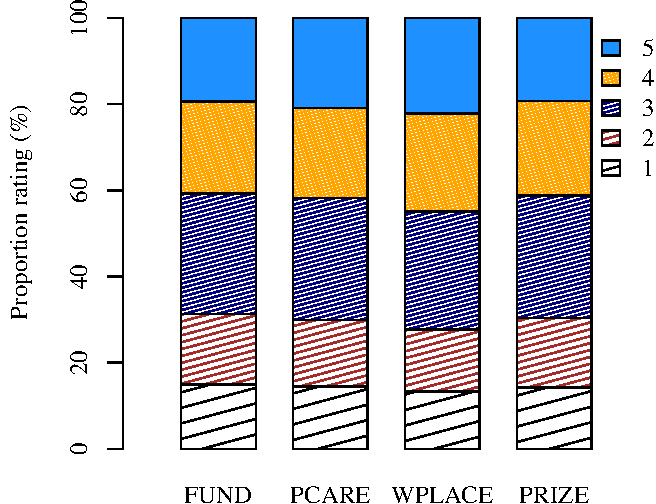
\includegraphics{figures/figure_ratings-1.pdf}
\end{figure}

The above analysis on the aggregate ratings does not hold in
general.\footnote{It crucially relies on the assumption that an
  increment in a proposal's quality as measured by an increase in
  ratings from \(v\) to \(v+1\) is the same for any value \(v\).} So, we
also examine the distribution of ratings as generated by treatments with
no aggregation. We have over 12,000 ratings, providing a very sensitive
test for differences across treatments. Using a Pearson's Chi-squared
test we find that the hypothesis of dependence between the distribution
of ratings and the treatments is \emph{not} quite significant at the 10
percent level (p-value of 0.103). Driving the p-value is a less than
\(2\) percent difference between the proportion of 5's in the WPLACE
treatment versus the other distributions, which is probably due to
outliers (the winning proposal was in the WPLACE treatment). Taken
together with the fact that our sample is large, we have strong evidence
suggesting that there are no (economically meaningful) differences in
the quality of project proposals across treatments and in particular no
evidence of a quantity versus quality trade-off up to the resolution of
the five-point scale.\footnote{One may worry that such binning is a
  fairly coarse measure of quality. In particular, effects concentrated
  in the upper tail of the distribution may not be detected. For
  example, compare the ratings of proposals A, B, C and D with
  hypothetical true qualities of 3, 4, 5, and 10 stars respectively.
  Under a five-point scale rating system, proposals A and B can be
  distinguished, but C and D cannot be distinguished. Hence, one needs
  to be very cautious in interpreting these results as evidence against
  quality effects in general.}

\emph{Quality assessed by managers.} One potential limit of assessing
quality only on the basis of peer ratings is that the employees might
have a different view of a proposal's quality than executives (due, for
instance, to a misalignment of incentives). Indeed, to ensure alignment
between managerial goals and the peer assessment, all project proposals
were further vetted by the HTL staff before being considered for
implementation funding. So, we now focus on the outcomes of this vetting
process to investigate more broadly the presence of treatment effects on
the quality of project proposals.

The vetting process conducted by the HTL staff resulted in 93 proposals
being scored (from 1 to 100 points) with the best 29 proposals invited
to submit implementation plans. The remaining 20 proposals were excluded
(and received a score of zero) either because flagged as inappropriate
for funding or because the proponent manifested no intention to
participate in the implementation phase (a Fisher's Exact Test for Count
Data finds no association between proposals excluded and treatments with
a p-value of 0.652).

The Spearman's rank correlation coefficient between the scores given by
the HTL staff and the average peer ratings was relatively high (0.198),
indicating good agreement between our two measures of quality. Indeed,
as before, we find no treatment effects on quality using the scores (a
Kruskal-Wallis rank sum test gives a p-value of 0.437). We also find no
treatment differences in the percentage of submitters being selected and
invited by HTL staff to present additional implementation plans (a
Fisher's Exact Test for Count Data gives a p-value of 0.652). Although
not significant, employees who made project proposals in the FUND
solicitation treatment are less likely to be selected as finalist than
the others (only 1 out of 7 in the FUND treatment were selected and
invited by the HTL staff), providing additional evidence of a no
quantity versus quality trade-off, as discussed before.

\subsection{The content of the project
proposals}\label{the-content-of-the-project-proposals}

The goal of the challenge was to improve Heart Center operations by
identifying problem areas and potential solutions. The proposed projects
broadly conformed to the stated goals of the contest, aligning with
improving the work processes within the organization or providing
high-quality patient care. For example, one project proposal that
received high peer ratings was to create a platform for patients to
electronically review and update their medicine list in the office prior
to seeing the physician. Another was to develop a smartphone application
showing a patient's itinerary for the day providing a guide from one
test or appointment to another. Nevertheless, other contest organizers
may have varying goals and be concerned about different aspects of the
submissions.

In order to examine additional dimensions of submission content, we now
study the area of focus of the submissions. Of particular interest is
understanding whether different wordings used in the general
encouragement solicitations (either towards improving the workplace or
targeting the wellbeing of patients) induce employees to concentrate on
different categories.

\begin{table}
\centering
\caption{Project proposals by area of focus}
\label{tab: area-of-focus}
\begin{tabular}{@{}lccccc}
  \\[-1.8ex]\hline \hline \\[-1.8ex]
 & FUND & PCARE & WPLACE & PRIZE & Total \\ 
  \hline \\[-1.86ex]
Information and access & 0 & 4 & 8 & 11 & 23 \\ 
  Patient support & 2 & 8 & 7 & 6 & 23 \\ 
  Care Coordination & 1 & 9 & 3 & 7 & 20 \\ 
  Staff workflow & 4 & 5 & 4 & 5 & 18 \\ 
  Workplace & 3 & 6 & 3 & 5 & 17 \\ 
  Quality and safety  & 0 & 0 & 5 & 5 & 10 \\ 
  Surgical tools and support to research & 1 & 1 & 0 & 0 & 2 \\ 
  [1.8ex] Total & 11 & 33 & 30 & 39 & 113 \\ 
   \\[-1.8ex]\hline \hline \\[-1.8ex]
\end{tabular}
\begin{tablenotes}
The areas of focus were manually identified by executives at the end of the competition for all the project proposals (due to a technical problem five proposals ended up with no classification).
\end{tablenotes}
\end{table}

Members of the HTL categorized each project proposal into one of seven
``areas of focus'' (Table \ref{tab: area-of-focus}): three categories
(``Care coordination'', ``Staff workflow'', ``Workplace'') identified
improvements for the workplace, other three (``Information and access'',
``Patient care'', and ``Quality and Safety'') focused on improvements
centered around patients, and another one (``Surgical tools and support
to research'') categorized projects developing tools to support
scientific research.

We test overall association between these categories and the
solicitation treatments with a Fisher's Exact Test for Count Data with
simulated p-value (based on 50000 replicates). Results show a marginally
significant (p=0.089) association, which means that our solicitation
treatments have indeed an effect on the content of the submitted
proposals.

To test which areas of focus was affected by our treatment, we regress
the probability of a project proposal being in a given category against
solicitation treatment dummies. We use an F-test where the null
hypothesis tested is that all the treatment effects have a zero effect
on the probability of the proposal being in a given category. The
results of these F-tests of overall significance (Table
\ref{areas of focus}) reveals significant differences in the ``Quality
and Safety'' and ``Information and access'' categories, which we view as
improvements centered around patients (as opposed to workplace
improvements). The first significance result is due to project proposals
in the PCARE solicitation treatment being less likely to fall in the
``Quality and Safety'' category. The second result is due to project
proposals in the FUND solicitation treatment being less likely to fall
in the ``Information and access'' category.

Although it is difficult to interpret these results because our model
does not provide any prediction on the content of proposals, they
indicate a possible trade-off between stimulating participation via
solicitations and inducing selection in the type of contributions to the
public good, which complicates the analysis of incentives for public
goods inside organizations beyond what the current literature
anticipates.

\begin{table}
\centering
\caption{Areas of Focus and Solicitation Treatment}
\label{areas of focus}
\begin{tabular}{@{}lcc}
  \\[-1.8ex]\hline \hline \\[-1.8ex]
 & F value & Pr($>$F) \\ 
  \hline \\[-1.86ex]
Patient support & 0.357 & 0.784 \\ 
  Information and access & 2.185 & 0.094 \\ 
  Quality and safety  & 2.512 & 0.062 \\ 
  Workplace & 0.751 & 0.524 \\ 
  Staff workflow & 1.291 & 0.281 \\ 
  Care Coordination & 1.284 & 0.283 \\ 
  Surgical tools and support to research & 1.660 & 0.180 \\ 
   \\[-1.8ex]\hline \hline \\[-1.8ex]
\end{tabular}
\end{table}

We also look at differences in the underlying complexity of the project
proposal as captured by differences in the length (i.e., the word count)
of a submission. Submissions were below 200 words in most cases with
little differences between the treatments. Indeed, testing for a
significant linear regression relationship between the length of
submissions and treatment dummies returned an overall insignificant
result (p=.43, F-test).

As a result, based on the analysis of the areas of focus and the length
of the submissions, we do find only little evidence of differences in
submission content across treatments. However, submission content is not
a well-defined concept and could be characterized in many dimensions.
While content does not vary in the dimensions we selected, we have not
exhausted all possible dimensions.

\subsection{Estimating social
preferences}\label{estimating-social-preferences}

The analysis above has shown that our solicitation treatments had both
positive and negative effect on participation, with no effects on
quality, and little sorting based on gender or profession. But what can
we say about the employees' preferences towards the common goal of
improving the organization?

In this section, we calibrate the theoretical model developed in Section
\ref{analytical-framework-and-predictions} with the experimental data to
get a sense of the magnitude of underlying preferences for contributing
to the organization. Following, the mixed-strategy equilibrium of the
model, the theoretical probability of contributing must be proportional
to the expected value of winning, \(R\), the underlying preferences
towards the public good, \(\gamma\), the marginal costs of contributing,
\(c\), and the number of agents, \(n\).

We assume the cost of making a submission \(c\) is the same in each
treatment,\footnote{This seems a reasonable assumption, given everyone
  is asked to perform the same task (identical submission procedure,
  same word limit, etc.).} and the individual preferences are constant,
being predetermined to our intervention. Then we derive a structural
relationship between the observed difference in the probability of
contributing \(\Delta p\) and the difference in the expected rewards
from winning \(\Delta R\) between the treatments.That is,\footnote{This
  equation can be obtained by following these steps. First, we
  approximate the profit equating condition \eqref{eq: mixed-strategy}
  to a linear function by noticing that the \(1/(1-(1-p)^n)\)
  approximates one for \(n\) large enough and \(p\) sufficiently small.
  Second, we solve for \(p\) and we simplify using the definitions of
  \(\Delta p\) and \(\Delta R\).}

\begin{equation}
  \Delta p \approx\frac{\Delta R}{n (c - \gamma)}.
\end{equation}

(Throughout this section we will consider \(\delta=0\) ignoring the
distinction between impure and pure altruism.) By solving for
\(\gamma\), we get

\begin{equation}
  \label{eq: gamma}
  \gamma   \approx  c -  \Delta R / (n\Delta p). 
\end{equation}

This implies that the parameter capturing individual preference for the
public good (that is consistent with our data) must be proportional to
the ratio between the difference in rewards and the difference in the
probability of submitting. Although we do not observe the levels of
\(R\) in each treatment, we approximate the difference of rewards
between the PRIZE and the other conditions by the pecuniary value of the
reward, which has its upper bound in the highest price that can be paid
for an iPad mini (\$350).\footnote{The price paid by the Heart Center
  was \$239 at the end of 2014 (including shipping cost). Other popular
  models (those with cellular data and large storage) could cost as high
  as \$350. Agents, however, were not aware of the specific model used
  for the competition and of the price paid. So, the value of \$350 is
  very conservative.} We further calibrate the cost of submitting a
proposal \(c\) to \$40 which is the median income per hour of a Nurse
Practitioner according to the Bureau of Labor Statistics; we assume the
number of competitors \(n\) to be 30 percent of the entire sample to
take into account rational expectations about the actual number of
participants in the contest.\footnote{This choice is our best guess of
  the number of active staff members at the Heart Center and is based on
  the number of employees who voluntarily took a survey before the
  experiment (378 people). Assuming greater participation would lead to
  artificially increasing the estimates of underlying incentives. In
  fact, staff members may have rational expectations about the actual
  number of potential participants, which may be less than the entire
  population.} Finally, by substituting these calibrated values into
equation \eqref{eq: gamma} along with the empirical difference in
participation rates between the PRIZE and the other treatments
(\(\Delta p=0.037\)), we get an estimate of the magnitude of the social
preferences towards the organization which is \(\hat\gamma=\$12\). As
shown in Figure \ref{fig: gamma}, this value is equivalent to about 30
percent reduction in the cost of contributing. Hence, increasing the
prize by \$100 is expected to raise the probability of submitting by 1
percentage points. This increase can be compared to the corresponding
increase of 0.7 that one will obtain by assuming no social preferences
\(\gamma=0\) at all.

\begin{figure} 
\centering
\caption{Estimated value of social preferences ($\hat\gamma$)}
\label{fig: gamma}
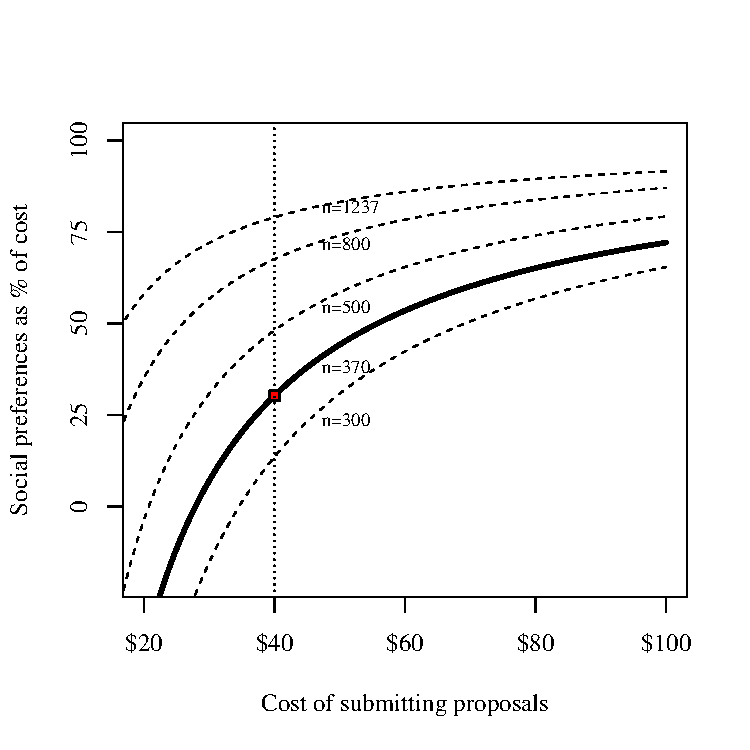
\includegraphics{figures/gamma-1.pdf}
\begin{tablenotes}
This figure plots the theoretical relationship between the cost of participation and the the social preferences parameter $\gamma$ (in percentage of the costs) which is consistent with our experimental data. Different curves represents different assumptions on the number of competitors. 
\end{tablenotes}
\end{figure}

A few remarks are in order here. To get confidence around these
estimates one need to consider several sources of uncertainty. First,
there is the uncertainty of estimating the probability of submitting in
our sample (standard errors can be computed directly from the data).
Another source of uncertainty is due to the calibration of the marginal
cost or the number of competitors. As shown in Figure \ref{fig: gamma},
the fraction of costs explained by social preferences increases
monotonically in the number of competitors (going up to 80 percent of
costs if employees expected to compete against every Heart Center staff
member); and decreases monotonically in the calibrated cost of making a
submission. Finally, another important source of uncertainty is
regarding the main behavioral assumptions of the model, as we discuss in
the next section.

\section{Summary and conclusions}\label{summary-and-conclusions}

We report results of a natural field experiment conducted at a medical
organization that held an innovation contest seeking contribution of
public goods (i.e., projects for organizational improvement) from its
more than 1200 employees. The experiment tested incentives for
contributing by manipulating the content of emails soliciting staff
participation. We presented different incentives to participate in the
contest, such as a prize (PRIZE) for winning submissions, improving
patient care (PCARE), improving the workplace (WPLACE), and funding for
implementation (FUND). Each staff was randomly assigned to receiving an
email containing one of the four incentives.

We find that the PRIZE solicitation treatment boosts participation by
about 40 percent relative to the WPLACE and PCARE solicitation
treatments. The FUND solicitation treatment is the least effective. It
generates not only about three times less submissions than the PRIZE
solicitation treatment, but also less submissions than the WPLACE and
PCARE solicitation treatments.

These participation differences, we find, are without changing the
quality of the submissions as judged by peers and the
management.\footnote{We find good agreement (high positive correlation)
  in the assessed quality of proposals between peer ratings and the
  evaluations conducted by the management; thus suggesting incentives
  being sufficiently aligned.} The higher employee participation in the
PRIZE solicitation treatment does not seem to be driven by low-quality
submissions. Similarly, the lower employee participation in the FUND
solicitation treatment does not seem to be driven by high-quality
submissions. In other words, treatments that attracted more (or less)
participation resulted in proposals of comparable quality and content.

Taken together, these findings suggest that (1) the
competition-for-prizes incentive dominates mission-oriented incentives
and (2) the opportunity to lead implementation of one's own submitted
project proposal is a poor incentive. In addition, these effects
combined with the small (extrinsic) value of the prize relative to the
median income of the participants, the long odds of winning the prize,
the lack of differences in participation among professions, and the
foreseeable additional costs of winning may suggest that (3) the effect
of a prize competition on participation goes beyond the actual value of
the prize itself, suggesting workers have, in fact, internalized some of
the benefits of participating in an organizational task.

We also fined that, although the WPLACE and PCARE solicitation
treatments are equally effective on average, responses appear sensitive
to the gender of the solicited person. Women's participation is greater
when emphasizing the patient care whereas men's participation is
significantly lower, controlling for the profession and position inside
the organization. This finding suggests that gender may be an important
factor influencing sensitivity of responses to solicitations concerning
the organizational mission.

At the same time, only an insignificant gender-based differences with
respect to participation in the PRIZE solicitation treatment was found:
women's participation was slightly higher but not significant than
men's, all else being equal. This evidence indicates that gender
differences in preferences, such as competitive inclinations or risk
aversion, may not exert great influence on responses of workers to
contests inside organizations.

We believe these results have three main implications for comparable
organizations and, more broadly, the internal provision of public goods.

The first implication is that announcing a competition for an individual
prize foster workers' participation in organizational tasks beyond the
value of the awarded prize itself. That is, prizes generate two opposing
externalities that help workers internalize the public good effects of
their organizational contributions. This result is important because it
highlights a relatively less understood function of contests that is to
mitigate the free riding incentives on organizational tasks.

A second implication is that offering the opportunity to lead collective
projects can exacerbate the free riding incentives. This result may
appear contrary to intuition. In theory, one may benefit more from
leading a project than winning an iPad. For instance, one may use the
opportunity to signal project management skills to the management aiming
for a career advancement; or steer some of the resources towards assets
or problems that are relatively more beneficial to his or her situation
compared to the rest of the organization. If so, why a negative result?
We believe that the private benefits from winning were negligible in our
setting. First, the opportunity for a career advancement is small
because medical staff gets promoted on the basis of other parameters
(e.g., the quality of care provided). Second, the peer evaluation and
vetting by the management ensure that the winning contributions yield as
distributed benefits as possible. These aspects may have eliminated the
possible private benefits from leading a project, resulting in poor
participation rates. This result is important because projects need to
be lead by someone and making more resources available does not seem to
increase volunteers.

A third implication is that participation in organizational tasks is
sometimes triggered by mission-based preferences. Although we find
evidence that these preferences can be an effective incentive, we also
find gender-based selection effects that are difficult to predict
ex-ante. Our experiment does not provide any insights to better
interpret these differences. But a large literature has investigated
gender-based difference in preferences \citep[see][ for a
review]{croson2009gender} or difference in self-stereotypes
\citep{coffman2014evidence} that could explain some of these effects.
Yet, more experimentation is needed to understand the different drivers
in the field inside organizations.

A few limitations of this study deserve consideration. The first is that
the validity of our causal interpretation of the results rests on a few
conventional assumptions \citep{rubin1974estimating}. These include the
``no interference between units'' assumption. In our study, it is
possible that communication among staff assigned to different treatment
arms could have influenced decisions to participate. The magnitude of
this interference would depend on intensity of staff communication and
the density of social interactions. Both of which should be small
because (i) an individual competition may provide only weak incentives
for information sharing and (ii) the staff members are scattered across
multiple buildings on the hospital campus. Even so, a potential
inference bias may alter the results towards a null effect as
differences in employee participation should converge towards zero when
communication spreads the content of the different email solicitations.
This goes against our results. Moreover, by looking at the temporal
dynamics of submissions, we find no indication of a convergence in the
participation rates. Hence, the assumption of no interference seems
appropriate.

Another potential limitation is that staff members may have left the
solicitation email that was sent to them unopened or unread, thus
non-complying with the assigned solicitation treatment. As this kind of
noncompliance is almost entirely unobserved,\footnote{The email was sent
  using the internal messaging system of the Heart Center, which, at the
  time, was not collecting individual analytics.} the analysis follows
an \emph{Intention-To-Treat} (ITT) approach, discarding entirely any
information about the solicitation treatment actually received. The main
drawback of an ITT analysis is that it does not answer questions about
causal effects of the content of the solicitation itself, only about
causal effects of the assignment to a solicitation treatment.

Finally, our results have implications that extend beyond the specific
organization under study. While the choice of focusing on health care
workers may limit the generalizability of our results in some respect,
it should be noted that in the US alone health care spending accounts
for 17 percent of the GDP (in 2015). And, more generally, our study
results are also directly applicable to a variety of other professions
exposed to a public good dilemma (e.g., teachers, public servants,
researchers). In all these settings, our study suggests that contests
soliciting employee contributions and awarding an individual prize to
the winning contribution appear an effective way to foster the internal
provision of public goods inside organizations.

\renewcommand\refname{References}
\bibliography{refs.bib}

\end{document}